
% 0213
% \textcolor{red}{
% We use NLTK tool~\footnote{\url{https://www.nltk.org/}} to separate the documents in these datasets into multiple sentences, and then add marks to the boundaries between sentences as positive samples and insert marks into the interval of single sentence to construct negative samples. 
% }
% \textcolor{red}{
% In a standard procedural document, a single sentence~(``If he/she needs dishes, then choose the desired dishes and specify the taste.'') may convey the information of multiple procedural fragments~(\ding{192}, \ding{193} and \ding{195}). To achieve this, we proceed to combine separated fragments in each group into cohesive aggregations using another boundary identification model. This model is trained on collected data from~\citet{castelli2020techqa, zhang-etal-2020-reasoning, lyu2021goal} that contain more fine-grained separated segments. 
% }
% Additionally, to include actor information of actions, we add the prefix "For somebody:" before fragments related to the actor. For instance, we add "For customer:" before fragments containing actions executed by the customer. 

% At this point, we can obtain preliminary document by concatenating all the aggregations. 
% However, such generated documents lack fluency because each fragment is transferred using a hand-written template. Hence, we utilize ChatGPT for rephrasing the documents, leveraging its demonstrated near or even superior human-level performance in rephrasing task~\cite{chui2023chatgpt}. 
% Despite this, it is possible that some redundant actions from the generated documents that were retained during the Decomposition \& Transformation process will still be present after rephrasing, and ChatGPT will inevitably make some mistakes during rephrasing process. To remove redundant actions and fix rephrasing errors, we further refine the generated documents by hand-writing rules and making manual corrections, ultimately obtaining a total of 3394 high-quality documents. The statistics of the constructed dataset is shown in Table~\ref{dataset:statistics}. 
% See appendix~\ref{app:SurfaceSmoothing} for more details. 
\section{Dataset}

% V1
% Research for the procedural graph extraction from text heavily relies on large-scale and high-quality datasets, which consist of procedural graph and document pairs. 
% However, annotating the procedural graph based on corresponding document is a time-consuming and laborious task~\cite{maqbool2019comprehensive, bellan2020qualitative}. 
% Affected by the high annotation cost, existing datasets suffer from problems including small scale, incomplete procedural and factual knowledge representation and coarse-grained annotation. 

% Comparing to manually annotating procedural graphs based on procedural documents, our approach is less expensive and more efficient to implement with the help of automatic text generation technologies~\cite{zhang2023survey}, allowing for the construction of large-scale and high-quality dataset. 
% Moreover, such approach can better ensure the quality of the procedure graphs, as the existing procedure graphs are constructed by a large number of domain experts, which consume a lot of resources and have been validated by those experts. 

% V2
% Annotating the procedural graph based on corresponding document is challenging and laborious~\cite{maqbool2019comprehensive, bellan2020qualitative}. To construct high-quality dataset at a low cost, inspired by Data2Text task~\cite{lin2023survey}, we propose to supplement procedural documents for existing procedural graphs using available resources~\cite{dumas2018fundamentals}. 

% To promote optimal procedural graphs extraction, we use the Business Process Model and Notation (BPMN)~\cite{dijkman2011business} graph as the original procedural graph data for procedural documents supplementation. BPMN is the most commonly used type of procedural graph both in industry and academia~\cite{lopes2023assessing}. It is capable of complete procedural and factual knowledge representation~\cite{kocbek2015business, corradini2018guidelines} and is more complex and challenging compared to simple procedural graph containing only sequential actions, such as workflow~\cite{pal2021constructing, ren2023constructing}. This can help to evaluate whether existing studies can deal with the extraction of procedural graphs with higher complexity, in addition to the small-scale datasets that existing studies focus on. 
% involving a wide range of fields

% BPMN graphs consist of complete representations of various procedures, including plenty of complex branches and crucial constraints~\cite{corradini2018guidelines}, thus pose much more challenges than those containing only sequential actions, such as workflow~\cite{ren2023constructing}. 

% \begin{figure*}[t]
%     \centering
%     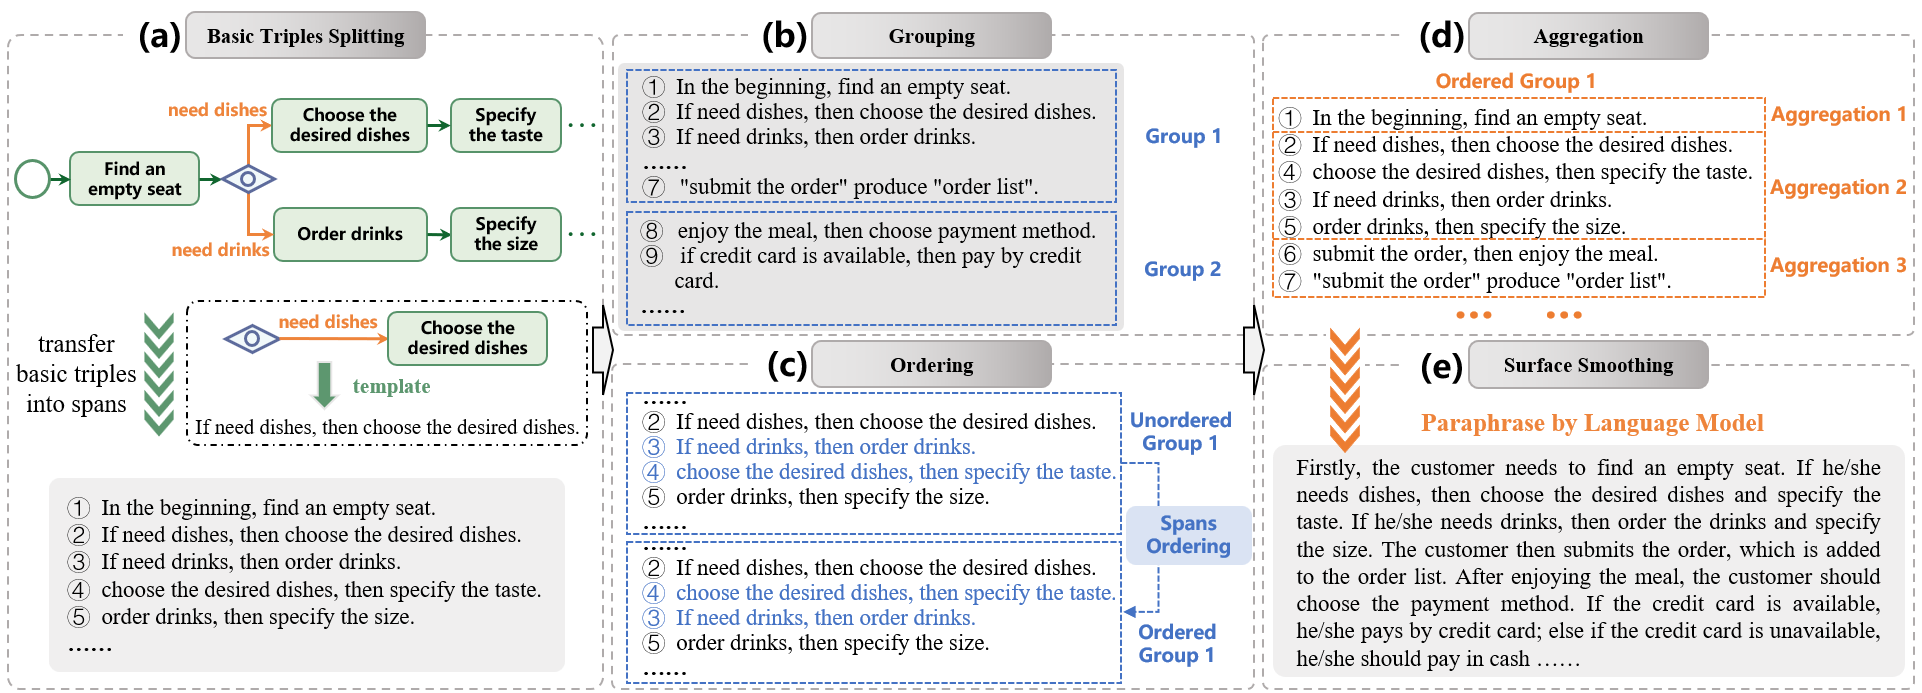
\includegraphics[width=\textwidth]{figures/DatasetConstruction.png}
%     \caption{The three-stage pipeline to supplement the procedural document based on the procedural graph.
%     }
%     \label{fig:DatasetConstruction}
% \end{figure*}

% V3
It is too costly to conduct an expert annotation of optimal procedural graphs for a large number of documents. As a remedy, we build our dataset upon a textbook~\cite{dumas2018fundamentals}, which has defined optimal procedural graphs covering the whole business process management lifecycle. In this way, the dataset construction turns into a data2text task --- generating a suitable document for a given procedural graph.
\subsection{Preliminary}
Figure~\ref{fig:task_b} presents an example of the optimal procedural graph. It describes the procedure of how a restaurant serves customers and involves two actors~(customer and restaurant). 
Each actor starts from the ``Start'' node, carries out actions following the logic in the graph, and ends at the ``End'' node. If the actions are performed sequentially, they are connected by the ``Sequence Flow''. Otherwise, there is an ``Inclusive Gateway'', ``Exclusive Gateway'' or ``Parallel Gateway'' indicating the following actions are non-sequential ones. Both the ``Inclusive Gateway''~(G-1) and ``Exclusive Gateway''~(G-3) mean that the following action is performed under the condition on the connected ``Condition Flow''. The difference is that there is one and only one condition after the ``Exclusive Gateway'' can be met, while this does not apply to the ``Inclusive Gateway''. The ``Parallel Gateway''~(G-5) represents that the following actions are performed in parallel. Note that, all gateways appear in pairs and the latter ones~(G-4, G-2, G-6) indicate the end of the non-sequential activities. Additionally, the ``Data Constraint'' and ``Action Constraint'' represent the necessary data~(C-1) and essential notices~(C-2) for actions connected by the ``Constraint Flow'', respectively.

% meaning the next action to be performed after the current condition is determined by specific conditions, 


% For each actor, starting from a ``Start'' notation, they execute the subsequent actions in the graph. Apart from simple sequential actions, the execution of non-sequential actions need to be represented by gateways. 
% % Gateway
% ``Exclusive Gateway''~(G-3) represents that the next action to be executed is determined by specific conditions. ``Inclusive Gateway''~(G-1) represents that one or more subsequent actions can be executed based on how many conditions are satisfied. 
% ``Parallel Gateway''~(G-5) represents the simultaneous execution of multiple actions. 
% % Constraint
% Additionally, ``Constraint'' represents the necessary data objects~(C-1) and essential notices~(C-2) for corresponding actions. 
% To integrate all elements and form a complete graph, ``Sequence Flow'' is used to connect different elements to show the progress of the procedure. Conditions used to determine executed non-sequential actions are represented by flows following exclusive and inclusive gateways. Furthermore, ``Constraint Flow'' links constraints with their corresponding actions. 

% 介绍图中的信息,主要是图例的定义和怎么看这个图
% \liang{xxxxxxxxxxxxx}
% As shown in Figure~\ref{fig:task_b}, the procedural graph starts from a 
\subsection{Dataset Construction}
With these high-quality procedural graphs, we then perform the dataset construction as a data2text task~\cite{lin2023survey}. Specifically, {we design a three-stage pipeline: 1) Decomposition \& Transformation that decomposes the graph into fragmented spans/sentences in natural language; 2) Grouping \& Ordering that logically organizes the procedural fragments; 3) Aggregating \& Smoothing that unifies the fragments into high-quality documents}. 

% Annotating procedural graph based on corresponding document is challenging and laborious~\cite{bellan2020qualitative}. To construct high-quality dataset at a low cost and promote optimal procedural graphs extraction, inspired by Data2Text task~\cite{lin2023survey}, we propose to build a dataset based on a business management textbook~\cite{dumas2018fundamentals}, which has summarized business processes into high-quality procedural graphs with complete sequential actions, non-sequential actions, and constraints. 

% Following ``easy to hard''~\cite{gao2023easy} strategy, we propose a three-stage pipeline to divide the document generation of an entire graph into manageable ones and solve them progressively, as shown in Figure~\ref{fig:DatasetConstruction}. 


% \liang{Check the comments here}
% 写作重点是要准确,不要写废话,只描述关键信息,对应图或者表中的例子,方法和实现步骤侧重描述我们针对本文任务做的特殊措施和改进
% 这部分写完了,改一版abstract出来,因为flow基本就可以定了,我们之后就算改了正文也可以只微调abstract了,控制20行左右


% 为了缩小直接从complex graph到length document之间的巨大gap,我们选择第一步将图分解为最小meaningful的单元,解释一些比较重要的定义,比如每个单元的第一个元素和最后一个元素不能是flow之类的,Note that 为了remain action之间的顺序或者约束?,哪些结点是重复遍历的,进一步为每个basic unit设计了template,这些template不一定是完整的句子,也可以是一些span,也费力去编写不同版本的template 只需要能够完整表达unit的意思就可以,我们把这些sentences/spans 统称为procedural fragments详细参见xxx

\begin{figure}[t]
    \centering
    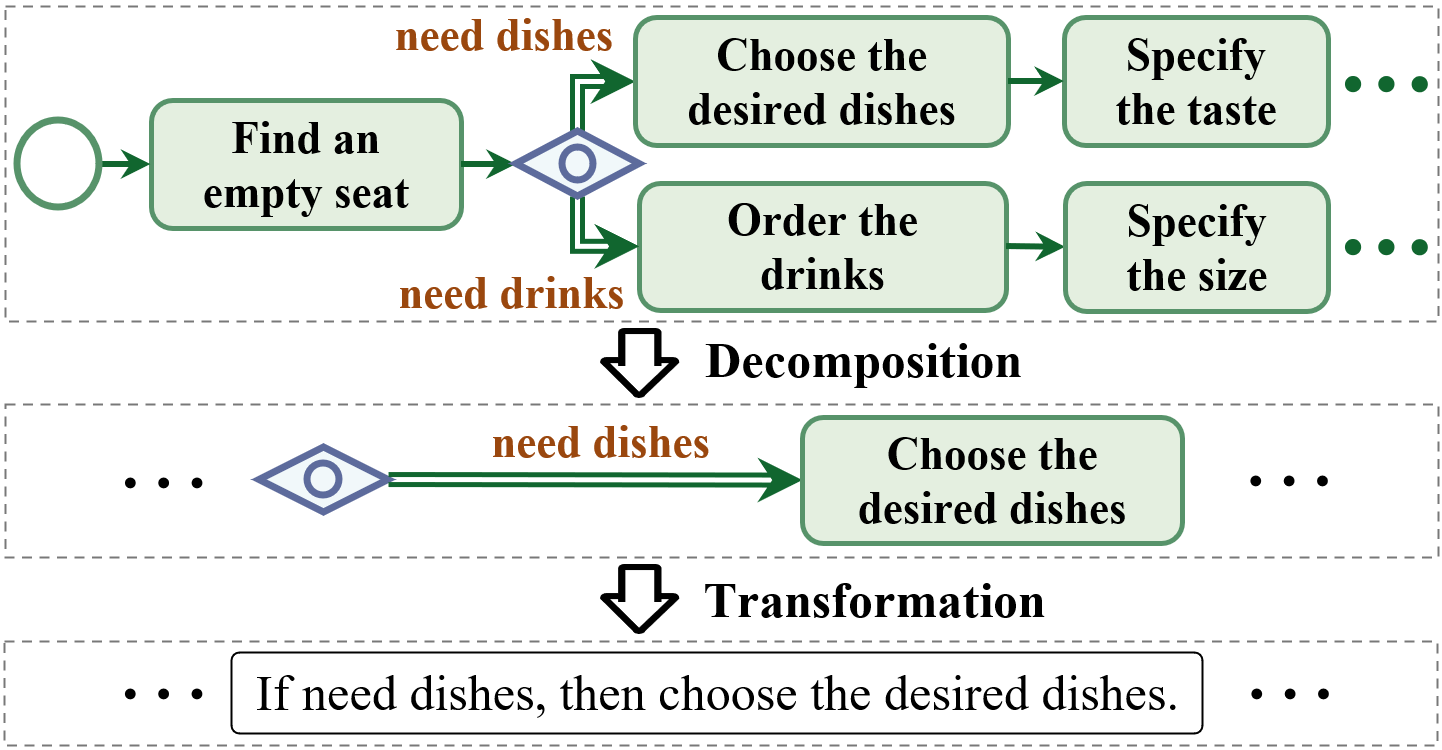
\includegraphics[width=\linewidth]{figures/dataset/DatasetConstruction_1.png}
    \caption{Example of Decomposition \& Transformation.
    }
    \label{fig:Decomposition}
\end{figure}
\paragraph{Decomposition \& Transformation}
To narrow the huge gap between the complex graph and the length document, we first decompose the graph into minimal meaningful units. We define a vocabulary with nineteen units, each of which consists of actions, gateways or constraints connected by flow~(cf., Appx.~\ref{app:TriplesSplitting}). We also design nineteen hand-written templates for the vocabulary. Based on the unit vocabulary, we perform the breadth-first search strategy~\cite{10.1016/0004-3702(85)90084-0} over the graph, as shown in Figure~\ref{fig:Decomposition}. Note that, some actions may be repeatedly walked to preserve the sequential execution relation between adjacent actions in the graph. For example, ``Order drinks'' is walked twice, forming ``If need drinks, then order drinks.'' and ``order drinks, then specify the size.''. We then transfer the decomposed units into natural language spans/sentences based on the paired templates. We call these spans/sentences ``procedural fragments''. 

% Inspired by xxxx(我随便找了一篇Summarization of Diagrams in Documents,还有一些托福考试博客https://ielts-up.com/writing/task-1-diagram.html,你可以再让liao找一些更有说服力的参考文献)为了describe the detailed fragment in a logic way, 我们首先讲fragments进行分组。解释具体是怎么做的。每一组xxx(这个组具体代表了什么,一个subgoal,或者连贯执行的action之类的,这个你自己思考下)。
%由于xxx(需要排序的原因,因为你生成unit的时候肯定是按照一定顺序,为什么这个顺序还需要重新排一下,而且为什么可以只做组内排序)我们还进行了组内排序。解释具体是怎么做的,我们把order完的组叫做AAA(要不要起名字看你的选择)
% \begin{figure}[t]
%     \centering
%     \subfigure[Grouping]{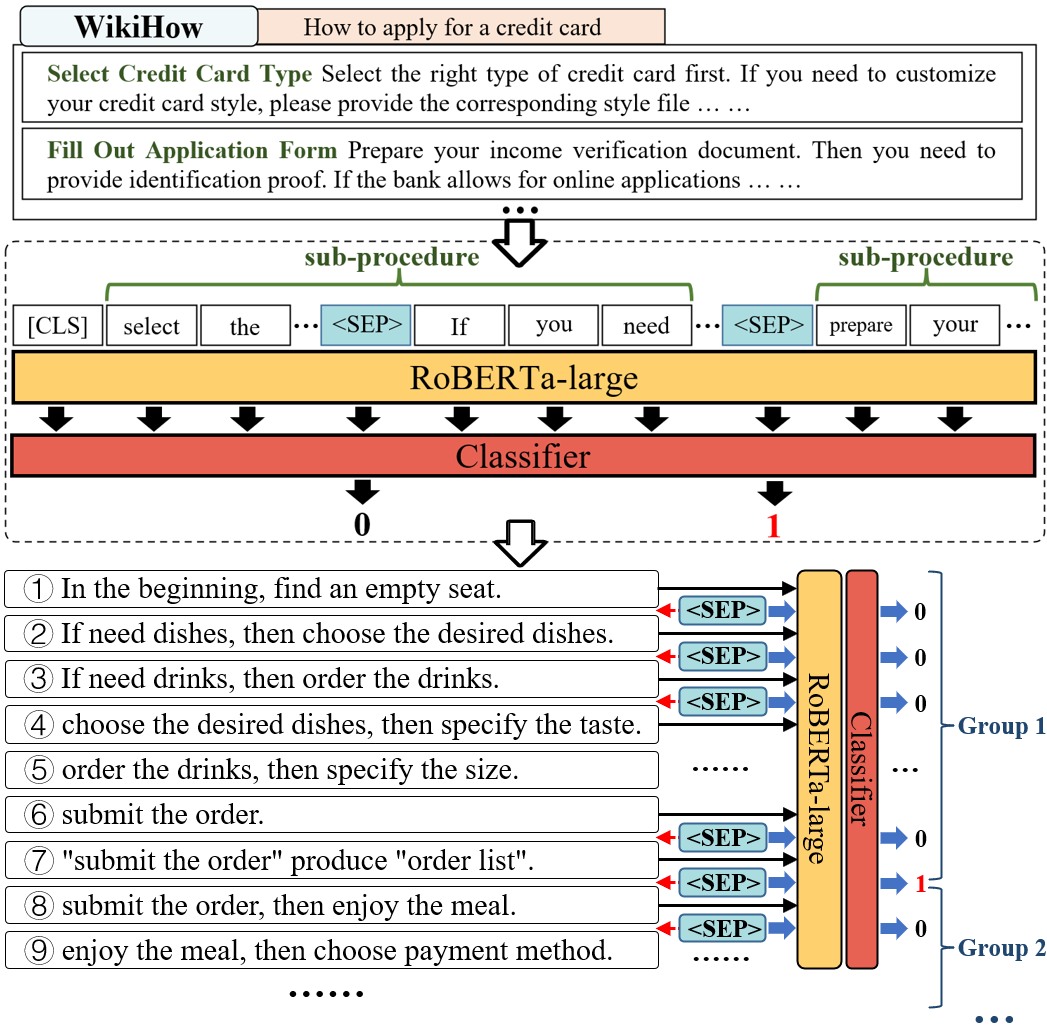
\includegraphics[width=\linewidth]{figures/dataset/DatasetConstruction_2.png}
%     \vspace{-0.5cm}
%     \label{fig:Grouping}}

%     \vspace{-0.2cm}
%     \subfigure[Ordering]{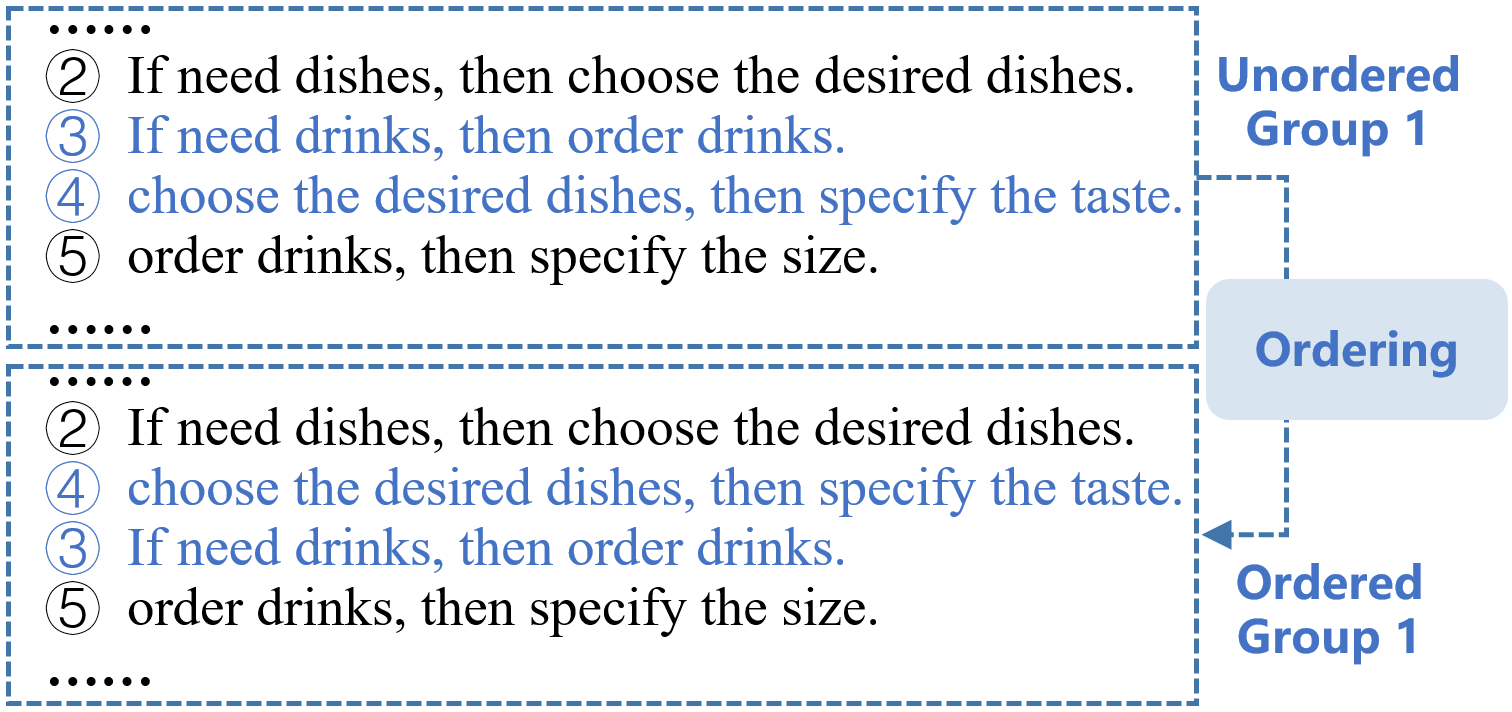
\includegraphics[width=\linewidth]{figures/dataset/DatasetConstruction_3.png}\label{fig:Ordering}}

%     \caption{Example of Grouping \& Ordering.
%     }
%     \label{fig:Grouping_Ordering}
% \end{figure}

\begin{figure}[t]
    \centering
    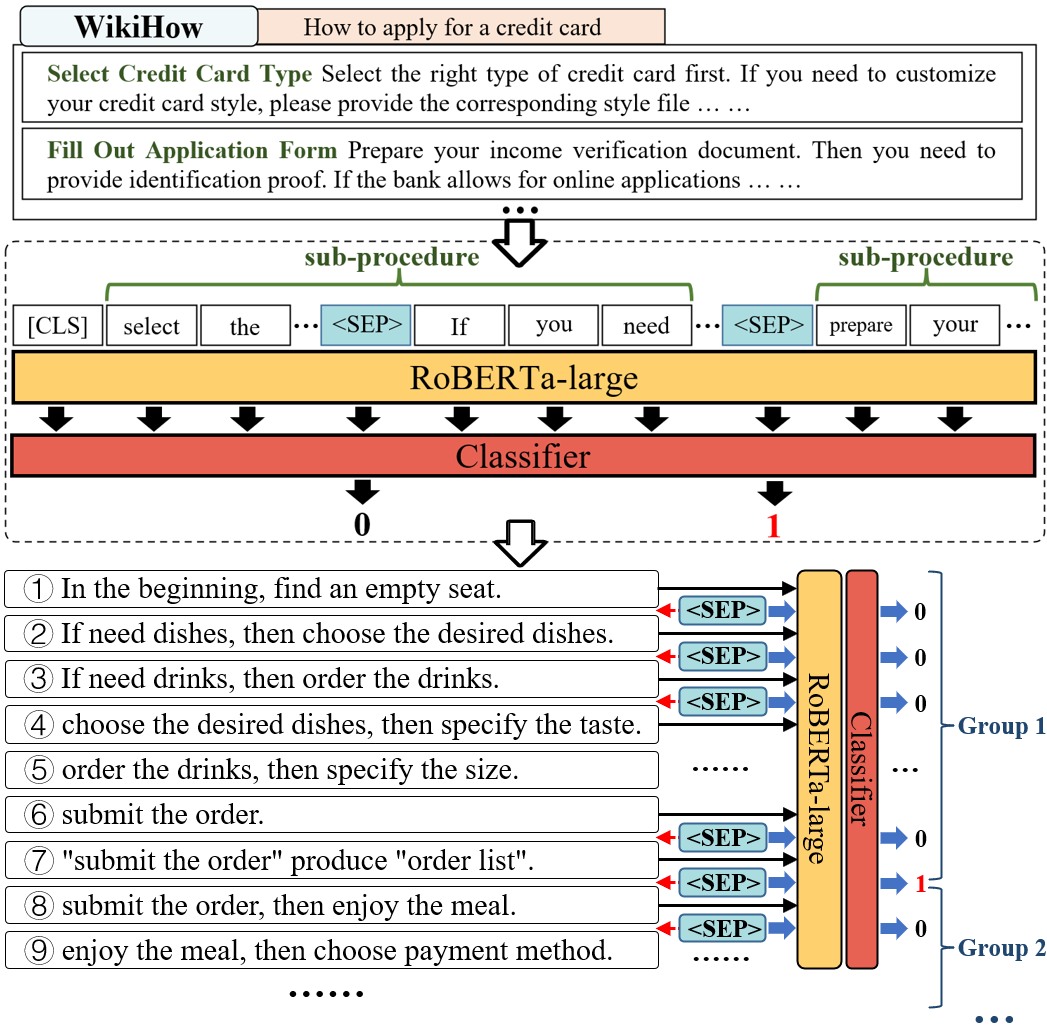
\includegraphics[width=\linewidth]{figures/dataset/DatasetConstruction_2.png}
    \caption{Example of Grouping \& Ordering.
    }
    \label{fig:Grouping_Ordering}
\end{figure}

\paragraph{Grouping \& Ordering}
When writing a procedural document, it is vital to provide information in a logical way, namely, describing the whole procedure sub-procedure by sub-procedure~\cite{futrelle1999summarization, futrelle2004handling}. Hence, we need to group the fragments into sub-procedures. We model this as a boundary identification task. Specifically, 
\textcolor{red}{
we train a boundary identification model using the WikiHow~\cite{bolotova2023wikihowqa} corpus that contains documents consist of numerous textual segments. We add separator token ``<SEP>'' between these segments to construct positive boundaries and insert separator tokens into the interval of the sentences within each segment to construct negative boundaries. A token classifier is then used to predict if each added separator token is a group boundary, allowing us to divide all fragments into different groups based on these predictions. 
}

% different groups using a boundary identification model. 
% Each group describes a sub-procedure of the whole procedure that is semantically coherent. 
% For example, we divide the customer's procedure before and after ``submit the order'' into two groups as shown in Figure~\ref{fig:Grouping_Ordering}. 
% We add a separator token ``<SEP>'' between every pair of adjacent fragments and employ a token classifier to predict the group boundaries of these fragments. 

\textcolor{red}{
After grouping, although the fragments in each group can together form a sub-procedure, the order that the algorithm traverses the graph not always aligns with how humans describe the actions in these fragments. 
For example, as shown in Figure~\ref{fig:Grouping_Ordering}, ``\ding{193}If need dishes, then choose the desired dishes'' should be immediately followed by ``\ding{195}choose the desired dishes, then specify the taste'', as only in this way, what the customer should do if meeting the condition ``need dishes'' can be continuously and coherently described. So we should order the fragments in Group1 to exchange the positions of fragment \ding{194} and \ding{195}. 
Therefore, we conduct fragments ordering within each group with a non-autoregressive ordering model~\cite{bin2023non}. 
We collect the data for model training from recent studies that provide off-the-shelf procedural documents consisting of sentences that describe a wide range of procedures~\cite{sakaguchi2021proscript, nandy2021question, bolotova2023wikihowqa}. We shuffle the sentences in the original documents and train the model to restore the order of these sentences. 
See appendix~\ref{app:NarrationAdjustment} for more details.}

% In a standard procedural document, 一些情况下,一个句子可以表述多个AAA. To achieve this, we xxx. 虽然到了这一步已经有了看似可以的document,但是由于模板的问题,这类document还不够流畅,所以我们利用Chatgpt, which has 在改写方面展现了接近甚至超越人类表现(citation),进行了润色。到这一步还没结束,因为一个好的procedural document应该是简洁而准确的---chatgpt并没有完全规避之前为了保证完整逻辑设置的重复节点的影响,文档仍存在一些冗余,同时由于chatgpt官方改写任务的特性,存在少量的错误修改。我们通过规则和人工校对进一步进行了xxx, 最终得到了高质量的document。
\paragraph{Aggregating \& Smoothing}
\textcolor{red}{
In a standard procedural document, a single sentence~(``If he/she needs dishes, then choose the desired dishes and specify the taste.'') may convey the information of multiple procedural fragments. To achieve this, we proceed to combine separated fragments in each group into cohesive aggregations using another boundary identification model. This model is trained on collected data from~\citet{castelli2020techqa, zhang-etal-2020-reasoning, lyu2021goal} that contain more fine-grained separated segments. 
}
Additionally, to include actor information of actions, we add the prefix "For somebody:" before fragments related to the actor. For instance, we add "For customer:" before fragments containing actions executed by the customer. 

At this point, we can obtain preliminary document by concatenating all the aggregations. 
However, such generated documents lack fluency because each fragment is transferred using a hand-written template. Hence, we utilize ChatGPT for rephrasing the documents, leveraging its demonstrated near or even superior human-level performance in rephrasing task~\cite{chui2023chatgpt}. 
Despite this, it is possible that some redundant actions from the generated documents that were retained during the Decomposition \& Transformation process will still be present after rephrasing, and ChatGPT will inevitably make some mistakes during rephrasing process. To remove redundant actions and fix rephrasing errors, we further refine the generated documents by hand-writing rules and making manual corrections, ultimately obtaining a total of 3394 high-quality documents. The statistics of the constructed dataset is shown in Table~\ref{dataset:statistics}. 
See appendix~\ref{app:SurfaceSmoothing} for more details. 


% \subsection{Basic Triple Splitting}
% \label{Splitting}
% To smooth out the gap between structured graph data and natural language text, we first split each procedural graph into basic triples according to the breadth first search~\cite{10.1016/0004-3702(85)90084-0} results of the graph, and then transfer them into natural language spans using hand-written templates. 
% For example, the triple ``(Inclusive gateway, need dishes, Choose the desired dishes)'' is transferred into ``If need dishes, then choose the desired dishes'' as shown in Figure~\ref{fig:DatasetConstruction}~(a). 
% See appendix~\ref{app:TriplesSplitting} for details. 

% \subsection{Narration Adjustment}
% \label{Narration Adjustment}
% % Due to the large amount of information contained in each procedure graph and the complex graph structure, simply concatenating all the transferred spans into single text may result in logical confusion and a lack of narrative hierarchy. To mimic the way humans describe the procedure graph, in which the entire graph is divided into different parts and described separately, we propose a three-step strategy to divide each graph into multiple groups and adjust the narrative order of the spans in each group. 

% % We adopt boundary identification methods and spans ordering models to adjust the narrative manner of the transferred spans for the entire graph. Through our elaborate adjustment, we are able to improve the semantic coherence of the generated text and the information consistency between the generated text and the original graph, as shown in Figure~\ref{}. 
% % For example, as shown in Figure~\ref{}, when encountering logical judgments, humans describe the situation of one branch first, and then go on to describe the remaining branches. 

% Simply concatenating all the transferred spans to form the document may result in confused expressions and the lack of coherence because inflexible templates are used. 
% To mimic the way humans describe the procedural graph, in which the entire graph is divided into different parts and described logically, we propose a ``Grouping-Ordering-Aggregating'' strategy to divide the spans of each graph into multiple groups, and adjust the narrative order and manner of the spans within each group. 
% See appendix~\ref{app:NarrationAdjustment} for details of adopted models and training corpus. 

% \paragraph{Grouping}
% % Instead of describing all the information in an entire graph continuously, humans divide the procedure graph into different parts and describe them one by one. 
% To improve the clarity and coherence of expressions for the generated documents, we use boundary identification model to divide the transferred spans into different groups. 
% For example, divide the customer's actions before and after ``submit the order'' into two groups as shown in Figure~\ref{fig:DatasetConstruction}~(b). 
% Inspired by \cite{narayan2017split}, we add a unique separator token ``<SEP>'' between every pair of adjacent spans and employ a token classifier to predict the group boundaries of each graph's spans. 
% % The predicted boundaries divide the spans into different groups for further transforming into fluent document. 

% \paragraph{Ordering}
% It is necessary to order the spans in each group because instead of describing the graph in the order that the algorithm traverses the graph in section~\ref{Splitting}, humans will adjust the narrative order of the information on the graph for clear and coherent expressions. 
% For example, as shown in Figure~\ref{fig:DatasetConstruction}~(c), ``If need dishes, then choose the desired dishes'' should be immediately followed by ``choose the desired dishes, then specify the taste'', as only in this way, what the customer should do if meeting the condition ``need dishes'' can be continuously and coherently described. 

% For effective spans ordering, we simultaneously utilize the non-autoregressive ordering model~\cite{bin2023non}, the autoregressive ordering model~\cite{calizzano2021ordering} and heuristic rules and compare their effectiveness later in section~\ref{Dataset Quality Evaluation} to determine the best one to use. 

% \paragraph{Aggregating}
% % To further improve the clarity of expression and narrative coherence of the generated document, we proceed with an aggregation process on the ordered spans. We combine separated spans into cohesive aggregations using with fine-grained boundary identification. By doing so, we can avoid confused expression of various procedural and factual knowledge through describing the generated document sentence by sentence. 

% After grouping and ordering, the spans in each group may still contain multifarious information, resulting in cumbersome expressions of each group. 
% Therefore, we proceed to combine separated spans in each group into cohesive aggregations using fine-grained boundary identification. 
% For example, as shown in Figure~\ref{fig:DatasetConstruction}~(d), we divide the spans of group~1 into three aggregations to coherently describe how the customer finds a seat, orders the dishes and drinks, and then submits the order. 
% Additionally, to include actor information in the original graphs, we prepend the text "For somebody:" before the spans corresponding to the actor, indicating that all subsequent actions in those spans are executed by that actor. For instance, we add "For customer:" before spans containing actions executed by the customer. 

% \subsection{Surface Smoothing}
% Due to the fact that the basic triples in the original graph are transferred by hand-written templates, the generated documents may appear mechanical for reading and are not as fluent as the text written by human. 
% As a result, as shown in Figure~\ref{fig:DatasetConstruction}~(e), we conduct rephrasing operation on the concatenation of the processed spans using large language model to smooth out the discontinuities between the spans and improve semantic coherence for the final generated document. We add the unique separator token ``<SEP>'' to indicate the group and aggregation boundaries of the spans for the rephrasing model, which can prompt the model to describe these spans coherently and clearly. Details are listed in the appendix~\ref{app:SurfaceSmoothing}. 


% eva
\subsection{Dataset Analysis}
% \section{Dataset Quality Evaluation}
\label{Dataset Quality Evaluation}

To verify the reliability of our constructed dataset, we conduct both automatic and human evaluations to evaluate: (1) whether the generated documents are consistent with the original graphs and (2) whether the generated documents read coherently and fluently. 
We further evaluate the generated documents that are directly rephrased by ChatGPT without grouping, ordering and aggregating process to demonstrate the effectiveness of our proposed three-stage pipeline. 

\begin{table}[t]
\caption{Automatic evaluation results of the generated documents. 
``pipeline'' refers to generated documents processed by the full three-stage pipeline, and ``direct rephrasing'' refers to generated documents that are directly rephrased by ChatGPT without grouping, ordering and aggregating process. 
}
\label{dataset_eva}
\centering
\scalebox{0.85}{
\begin{tabular}{|l|c|c|}
\hline
\multicolumn{1}{|c|}{\textbf{Metric}} & pipeline & direct rephrasing \\ \hline
FINE-omission                         & 0.9049            & 0.8842            \\ \hline
FINE-hallucination                    & 0.9103            & 0.8838            \\ \hline
ESA-entity                            & 0.9707            & 0.9663            \\ \hline
ESA-action                            & 0.9648            & 0.9573            \\ \hline
\end{tabular}
}
\end{table}

% Please add the following required packages to your document preamble:
% \usepackage{multirow}
\begin{table}[]
\caption{Human evaluation results of the generated procedural documents.
}
\label{dataset_human}
\centering
\scalebox{0.75}{
\begin{tabular}{|l|cc|cc|cc|}
\hline
\multicolumn{1}{|c|}{\multirow{2}{*}{\textbf{Criterion}}} & \multicolumn{2}{c|}{pipeline}     & \multicolumn{2}{c|}{direct rephrasing} & \multicolumn{2}{c|}{direct concatenating} \\ \cline{2-7} 
\multicolumn{1}{|c|}{}                                    & \multicolumn{1}{c|}{Score} & ICC  & \multicolumn{1}{c|}{Score}    & ICC    & \multicolumn{1}{c|}{Score}     & ICC      \\ \hline
Understandable                                            & \multicolumn{1}{c|}{4.51}  & 0.93 & \multicolumn{1}{c|}{4.33}     & 0.89   & \multicolumn{1}{c|}{3.59}      & 0.92     \\ \hline
Adequacy                                                  & \multicolumn{1}{c|}{4.57}  & 0.94 & \multicolumn{1}{c|}{4.37}     & 0.91   & \multicolumn{1}{c|}{4.02}      & 0.89     \\ \hline
Hallucination                                             & \multicolumn{1}{c|}{4.59}  & 0.92 & \multicolumn{1}{c|}{4.47}     & 0.89   & \multicolumn{1}{c|}{4.11}      & 0.93     \\ \hline
Coherence                                                 & \multicolumn{1}{c|}{4.49}  & 0.90 & \multicolumn{1}{c|}{4.05}     & 0.90   & \multicolumn{1}{c|}{3.17}      & 0.89     \\ \hline
Humanness                                                 & \multicolumn{1}{c|}{4.43}  & 0.92 & \multicolumn{1}{c|}{4.31}     & 0.92   & \multicolumn{1}{c|}{2.86}      & 0.90     \\ \hline
\end{tabular}
}
\end{table}

% \begin{figure}[t]
%     \centering
%     \begin{minipage}{0.45\linewidth}
%         \centering
%         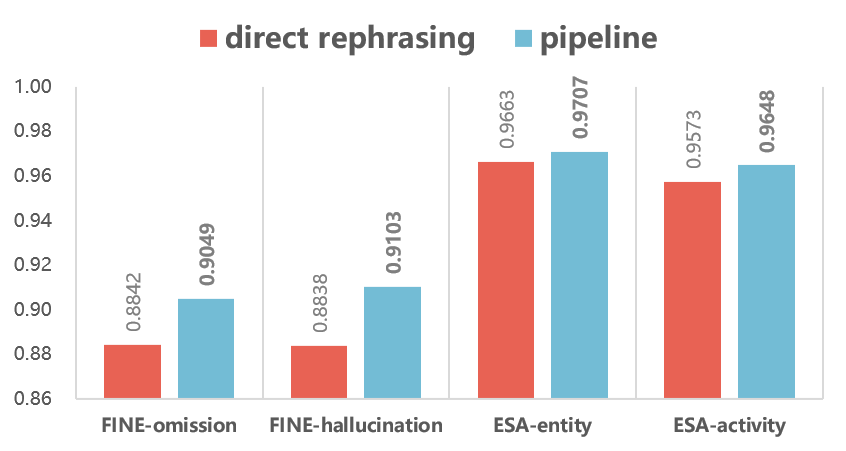
\includegraphics[width=\textwidth]{figures/dataset/DatasetEva.png}
%         \caption{Automatic evaluation results of the generated procedural documents. "non-auto" refers to non-autoregressive ordering model, "auto" to autoregressive ordering model, and "heuristic" to heuristic rules.}
%         \label{fig:DatasetEva}
%     \end{minipage}
%     \hfill
%     \begin{minipage}{0.45\linewidth}
%         \centering
%         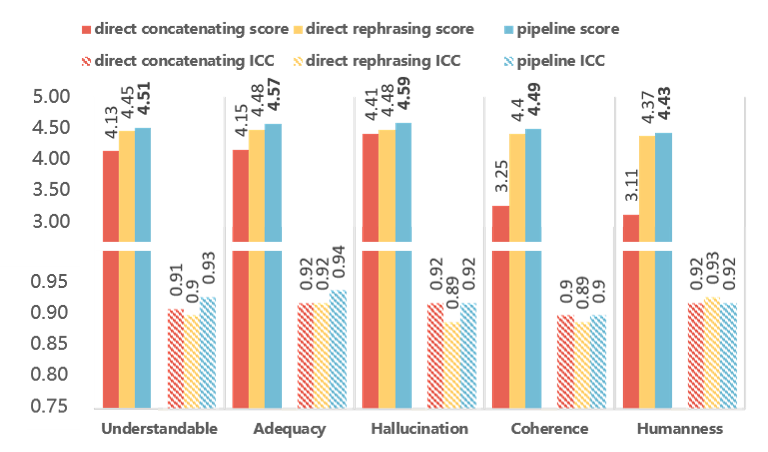
\includegraphics[width=\textwidth]{figures/dataset/DatasetHuman.png}
%         \caption{Human evaluation results of the generated procedural documents by different ordering approaches.}
%         \label{fig:DatasetHuman}
%     \end{minipage}
% \end{figure}

% \begin{figure}[t]
%     \centering
%     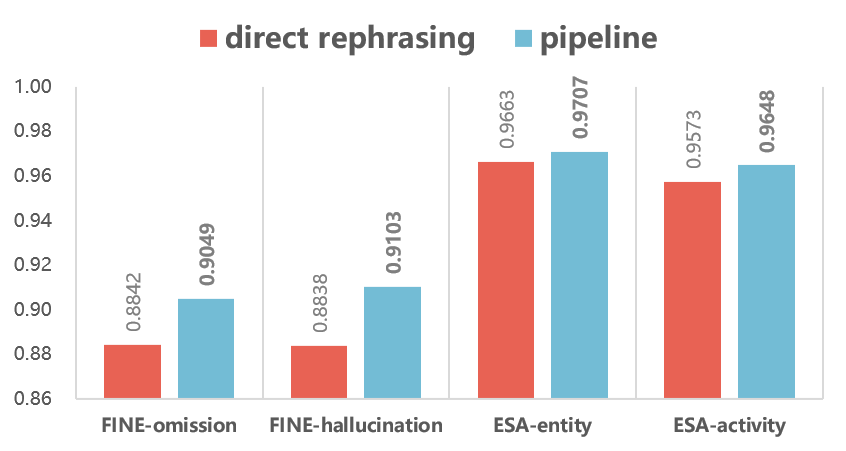
\includegraphics[width=\linewidth]{figures/dataset/DatasetEva.png}
%     \caption{Automatic evaluation results of the generated procedural documents. ``non-auto'' refers to non-autoregressive ordering model, ``auto'' refers to autoregressive ordering model and ``heuristic'' refers to heuristic rules.
%     }
%     \label{fig:DatasetEva}
% \end{figure}

\paragraph{Automatic Evaluation}
Following the evaluation strategies commonly used in Data2Text task~\cite{lin2023survey}, we adopt \textbf{FINE}~\cite{duvsek2020evaluating} and \textbf{ESA}~\cite{faille2021entity} to evaluate whether the generated documents fully cover the original graphs' information~(FINE-omission) and not contain redundant information~(FINE-hallucination), and maintain the entities and actions in the generated documents consistent with those in the original graphs~(ESA-entity \& action). 

As shown in Figure~\ref{fig:DatasetAuto}, evaluation results demonstrate that the generated documents processed by the full three-stage pipeline can achieve high consistency with the original graphs. The documents directly rephrased by ChatGPT fail to maintain high consistency as simply concatenate all fragments together can not present the information of the procedural graphs in a logic way, resulting in poor alignment between the generated documents and the original graphs. 

% As shown in Table~\ref{dataset_eva}, evaluation results demonstrate that both non-autoregressive and autoregressive ordering models can achieve high consistency with the original graphs. Heuristic rules fail to maintain high consistency as hand-written rules cannot cover various graph structures, resulting in incoherence of the generated documents.  


% \begin{figure}[t]
%     \centering
%     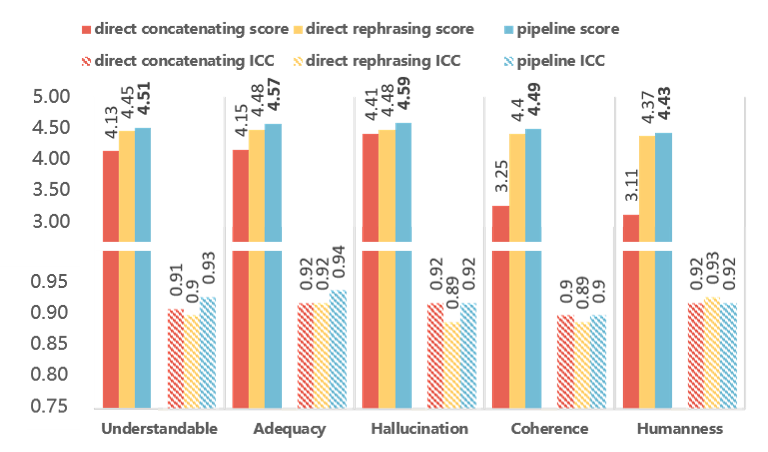
\includegraphics[width=\linewidth]{figures/dataset/DatasetHuman.png}
%     \caption{Human evaluation results of the generated procedural documents by different ordering approaches.
%     }
%     \label{fig:DatasetHuman}
% \end{figure}

\paragraph{Human Evaluation}
\begin{table}[!th]
\caption{Statistics of the constructed dataset. We present statistical information on the number of documents and various elements in the dataset.}
\label{dataset:statistics}
\centering
\scalebox{0.79}{
\begin{tabular}{|c|c|cc}
\hline
\textbf{Statistics} & \textbf{Num} & \multicolumn{1}{c|}{\textbf{Statistics}} & \multicolumn{1}{c|}{\textbf{Num}} \\ \hline
Document            & 3394         & \multicolumn{1}{c|}{Data Constraint}     & \multicolumn{1}{c|}{3500}         \\ \hline
Sentence            & 37226        & \multicolumn{1}{c|}{Action Constraint}   & \multicolumn{1}{c|}{2307}         \\ \hline
Token               & 566639       & \multicolumn{1}{c|}{Sequence Flow}       & \multicolumn{1}{c|}{36438}        \\ \hline
Action              & 36537        & \multicolumn{1}{c|}{Condition Flow}      & \multicolumn{1}{c|}{10598}        \\ \hline
Exclusive Gateway   & 7024         & \multicolumn{1}{c|}{Constraint Flow}     & \multicolumn{1}{c|}{5807}         \\ \hline
Inclusive Gateway   & 1204         & \multicolumn{1}{c|}{Actor}               & \multicolumn{1}{c|}{22775}        \\ \hline
Parallel Gateway    & 2050         & \multicolumn{1}{l}{}                     & \multicolumn{1}{l}{}              \\ \cline{1-2}
\end{tabular}
}
\end{table}

% To comprehensively evaluate the quality of the generated documents, we conduct human evaluation between the generated documents and the original graphs. 
We design five criteria to evaluate the generated documents through the rating of three experts, listed as follows:

\begin{itemize}
    \item \textbf{Understandable}: the generated document is capable of being understood. 
    \item \textbf{Adequacy}: the generated document fully covers all the information in the original graph. 
    \item \textbf{Hallucination}: the generated document does not contain any other information beyond the original graph. 
    \item \textbf{Coherence}: expressions of the generated document are coherent. 
    \item \textbf{Humanness}: the generated document reads like it was written by humans. 
\end{itemize}

\noindent
evaluators are required to rate each criterion on a scale of $1$ to $5$, with $5$ indicating that the generated document fully meets the requirements and $1$ indicating that it does not meet the requirements at all. 
We also report the ICC~(Intraclass Correlation Coefficient)~\cite{shrout1979intraclass} score to ensure the consistency between different evaluators and the evaluation effectiveness. Generally an ICC of $0.75$ or higher indicates that the evaluation is reliable~\cite{koo2016guideline}. 
% We report the average rating scores of different ordering approaches and the ICC scores in Table~\ref{dataset_human}. 

As shown in Table~\ref{fig:DatasetHuman}, 
the full three-stage pipeline can produce high-quality documents that are fluent and can achieve high equivalency with the original graphs. The generated documents directly rephrased by ChatGPT achieve lower scores that that processed by the full three-stage pipeline, because they fail to logically and coherently describe the procedural graphs, resulting in confusing expressions and incoherence of the generated documents. 
This indicates that it is necessary to group the fragments into sub-procedures, order the fragments within each group and combine separated fragments into cohesive aggregations, finally obtain high-quality documents. 

% We adopt the proposed three-stage pipeline and selected strategies to generate the procedural description text of corresponding raw procedure graph, and finally construct a total of 3394 samples, each with a pair of procedure graph and corresponding procedural description text. 
% The statistics of the dataset for our proposed benchmark \benchmark compared with the existing datasets for procedure graph extraction task is shown in Table~\ref{datasets}. 
